\def\documentauthor{Carlos Salinas}
\def\documenttitle{MA598: Lie Groups}
\def\shorttitle{MA544 Lie Groups}
\def\coursename{MA544}
\def\documentsubject{lie groups}
\def\authoremail{salinac@purdue.edu}

\documentclass[10pt,showtrims,twoside]{memoir}
\usepackage{geometry}
\usepackage[dvipsnames]{xcolor}
\usepackage[
    breaklinks,
    colorlinks=true,
    linkcolor=black,
    citecolor=black,
    filecolor=black,
    menucolor=black,
    runcolor=black,
    urlcolor=black,
    pdftitle={\shorttitle},
    pdfauthor={\documentauthor},
    pdfkeywords={\documentsubject},
    pdfsubject={\coursename}
    ]{hyperref}
\usepackage{natbib}

% TOC depth
\setsecnumdepth{subsection}

%% Math
\usepackage{amsmath}
\usepackage{amsfonts}
\usepackage{amssymb}
\usepackage{amsthm}
% \usepackage{mathtools}
% \usepackage{lmodern}
% \usepackage{eucal}

%% Language
% \usepackage[LAE,LFE,T2A,T1]{fontenc}
% \usepackage[utf8]{inputenc}
% \usepackage[farsi,french,german,spanish,russian,english]{babel}
% \babeltags{fr=french,
%            de=german,
%            en=english,
%            es=spanish,
%            pa=farsi,
%            ru=russian
%            }
% \def\spanishoptions{mexico}

% \selectlanguage{english}

% \newcommand{\textfa}[1]{\beginR\textpa{#1}\endR}

% \usepackage{CJKutf8}
% \newcommand{\textkr}[1]{\begin{CJK}{UTF8}{mj}#1\end{CJK}}
% \newcommand{\textjp}[1]{\begin{CJK}{UTF8}{min}#1\end{CJK}}
% \newcommand{\textzh}[1]{\begin{CJK}{UTF8}{bsmi}#1\end{CJK}}

%% Misc
\usepackage{graphicx}
\graphicspath{{figures/}}

\usepackage{microtype}
\usepackage{lineno}
\usepackage{multicol}
\usepackage[inline]{enumitem}
\usepackage{listings}
% \usepackage{mleftright}
% \mleftright
\usepackage{carlos-variables}

%% Unicode math
\usepackage{unicode-math}

% \setmainfont[Ligatures=TeX]{Latin Modern Roman}
% \setsansfont{Latin Modern Sans}
% \setsansfont{Latin Modern Mono}
% \setmathfont{Latin Modern Math}

%% Theorems and definitions
\theoremstyle{plain}
\newtheorem{theorem}{Theorem}
\newtheorem{proposition}[theorem]{Proposition}
\newtheorem{corollary}[theorem]{Corollary}
\newtheorem{claim}[theorem]{Claim}
\newtheorem{lemma}[theorem]{Lemma}
\newtheorem{axiom}[theorem]{Axiom}

\newtheorem*{corollary*}{Corollary}
\newtheorem*{claim*}{Claim}
\newtheorem*{lemma*}{Lemma}
\newtheorem*{proposition*}{Proposition}
\newtheorem*{theorem*}{Theorem}

\theoremstyle{definition}
\newtheorem{definition}{Definition}
\newtheorem{example}{Examples}
\newtheorem{examples}[example]{Example}
\newtheorem{exercise}{Exercise}[subsection]
\newtheorem{problem}[exercise]{Problem}

\newtheorem*{example*}{Example}
\newtheorem*{exercise*}{Exercise}
\newtheorem*{problem*}{Problem}

\begin{document}

%% Footnote style
\renewcommand*{\thefootnote}{\fnsymbol{footnote}}

%% Counters
\counterwithout{exercise}{chapter}
\numberwithin{equation}{subsection}
\counterwithout{equation}{chapter}

\thispagestyle{empty}
\author{\href{mailto:\authoremail}{\documentauthor}}
\title{\documenttitle}
\date{\today}

\frontmatter
\maketitle
\tableofcontents

%% Notes
\mainmatter
% \chapter{Prologue}
This summer, we will be making our way through Fulton and Harri's
\emph{Representation Theory} with applications to Lie groups, although we
will also reference Knapp's \emph{Lie Groups Beyond an Introduction}
\cite{knapp} and Milne's \emph{Lie Algebras, Algebraic Groups, and Lie
  Groups} \cite{milneLAG}. The goal is to eventually look at volume forms on

\begin{tabular}{cl}
  $C_n$  & is the cyclic group of order $n$ not necessarily equal
           (but isomorphic) to $\bbZ/p\bbZ$\\
  $S_n$ & is the symmetric group on $\{1,\dotsc,n\}$\\
  $A_n$ & is the alternating group on $\{1,\dotsc,n\}$\\
\end{tabular}

\newpage
\chapter{Representation Theory}
This section of the notes correspond to the first three chapters of Fulton
and Harris's book \emph{Representation Theory}. We will quickly talk about
the representation theory of finite groups and move on to the
representation theory of Lie groups in the next chapter.
\section{Representation of Finite Groups}
\subsection{Definitions}
Throughout this section, by a \emph{representation} of a finite group $G$
we mean a homomorphism $\rho\colon G\to\GL(V)$, where $V$ is a
finite-dimensional complex vector space. A \emph{representation} of a
finite group $G$ on a finite-dimension; we say that such a map $\rho$
\emph{gives $V$ a $G$-module structure.} When there is little ambiguity
about the map $\rho$, we will call $V$ itself a representation of $G$; we
also suppress the symbol $\rho$ and write $gv$ for $\rho(g)(v)$
whenever context allows us. The dimension of $V$ is called the \emph{degree} of
$\rho$.

A map $\varphi$ between two representations $V$ and $W$ of $G$ is a vector
space map $\varphi\colon V\to W$ such that
\[
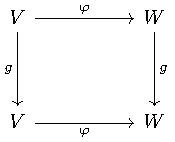
\includegraphics{figures/week-1-diag-1}
\]
commutes for every $g\in G$. We will call such a map a \emph{$G$-linear
  map} when we want to distinguish it from an arbitrary linear map between
the vector spaces $V$ and $W$. We can thus, then define $\Ker\varphi$,
$\Img\varphi$, and $\Coker\varphi$, which naturally inherit a $G$-module
structure from $V$.

A \emph{subrperesentation} of a representation $V$ is a vector subspace $W$
of $V$ which is invariant under the action by $G$, that is,
$gw=w$ for all $w\in W$. A representation $V$ is called
\emph{irreducible} if there is no proper nonzero invariant subspace $W$ of
$V$.


As it turns out, some of if $V$ and $W$ are representations, so are
$V\oplus W$ and $V\otimes W$ with $g(v\otimes w)\coloneq gv\otimes gw$,
and so are the $n$th tensor power $\bigotimes^nV$, the exterior power
$\bigwedge^n V$ and the symmetric powers $\Sym^n V$. The dual
$V^*=\Hom(V,\bbC)$ of $V$ is also a representation, though not in the most
obvious way: We want the two representations of $G$ with respect to the
natural pairing between $V$ and $V^*$, that is,
$\langle v^*,v\rangle\coloneq v^*(v)$, so that if
$\rho\colon G\to\GL(V)$ is a representation and $\rho^*\colon G\to\GL(V)$
is its dual, then we have
\[
  \langle \rho^*(g)(v^*),\rho(g)(v) \rangle=\langle v^*,v \rangle
\]
for all $g\in G$, $v\in V$, and $v^*\in V^*$. This in turn forces us
to define the dual representation $\rho^*\colon V^*\to V^*$ by
\[
  \rho^*(g)\coloneq{}^{\rmt}{\rho}(g^{-1})
\]
for all $g\in G$. Let us verify that $\rho^*$ in fact satisfies $\langle
\rho^*(g)(v^*),\rho(g)(v) \rangle=\langle v^*,v \rangle$: Let
$v^*\in V^*$ and $v\in V$,
then
\begin{align*}
  \langle\rho^*(g)(v^*),\rho(g)(v)\rangle
  &=\langle{}^\rmt\rho(g^{-1})(v^*),\rho(g)(v)\rangle\\
  &=\langle v^*,\rho(g^{-1})\circ\rho(g)(v)\rangle\\
  &=\langle v^*,v\rangle.
\end{align*}

Having defined the dual representation of the tensor product of two
representations, it is likewise the case that if $V$ and $W$ are
representations, then $\Hom(V,W)$ is also a representation, via the
identification $\Hom(V,W)=V^*\otimes W$. Unraveling this, if we view an
element of $\Hom(V,W)$ as a linear map $\varphi$ from $V$ to $W$, we have
\[
(g\varphi)(v)=g\varphi(g^{-1}v)
\]
for all $v\in V$. In other words, the definition is such that the diagram
\[
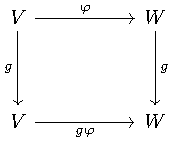
\includegraphics{figures/week-1-diag-2}
\]
commutes. Note that the dual representation is, in turn, a special case of
this: When $W=\bbC$ is the trivial representation, i.e., $gw=w$ for all
$w\in\bbC$, this makes $V^*$ into a $G$-module, with
$g\varphi(v)=\varphi(g^{-1}v)$, i.e.,
$g\varphi={}^\rmt(g^{-1})$.

\begin{exercise}
We verify that in general the vector space of $G$-linear maps between two
representations $V$ and $W$ of $G$ is just the subspace $\Hom(V,W)^G$ of
elements of $\Hom(V,G)$ fixed under the action of $G$. We will often denote
this space by $\Hom_G(V,W)$.
\end{exercise}
\begin{proof}
\end{proof}

We have taken the identification $\Hom(V,W)=V^*\otimes W$ as the
definition of the representation $\Hom(V,W)$. More generally, the usual
identities for vector spaces are also true for representations, e.g.,
\begin{align*}
V\otimes(U\oplus W)&=(V\otimes U)\oplus(V\otimes W)\\
\bigwedge^k(V\oplus W)&=\bigoplus_{a+b=k}{\textstyle\bigwedge^a V\otimes\bigwedge^b
  W}\\
{\textstyle\bigwedge^k V^*}&=\left({\textstyle{\bigwedge^kV}}\right)^*
\end{align*}

If $X$ is any finite set and $G$ acts on the left on $X$, i.e.,
$G\to\Aut(X)$ is a homomorphism to the premutation group of $X$, there is
an associated permutation representation: Let $V$ be the vector space with
basis $\{e_x:x\in X\}$, and let $G$ act on $V$ by
\[
  g\cdot\sum a_xe_x\coloneq\sum a_xe_{gx}.
\]
The regular representation, denoted $R_G$ or simply $R$, corresponds to the
left action of $G$ on itself. Alternatively, $R$ is the space of
complex-valued functions on $G$, where an element $g\in G$ acts on a
function $\alpha$ by $(g\alpha)(h)=\alpha(g^{-1}h)$.

\subsection{Complete Reducibility; Schur's Lemma}
Before we begin classifying the representations of a finite group $G$ we
should try to simplify life by restricting our search
somewhat. Specifically, we have seen that representations of $G$ can be
built up out of other representations by linear algebraic operations, most
simply by taking the direct sum. We should focus, then, on representations
that are ``atomic'' with respect to this operation, i.e., that cannot be
expressed as a direct sum of others; the usual term for such a
representation is \emph{indecomposable}. Happily, this situation is as nice
as it could possibly be: A representation is atomic in this sense if and
only if it is irreducible (i.e., contains no proper subrepresentations);
and every representation is the direct sum of irreducibles, in a suitable
sense uniquely so. The key to all this is
\begin{proposition}
If $W$ is a subrepresentation of a representation $V$ of a finite group
$G$, then there is an elementary invariant subspace $W'$ of $V$, so that
$V=W\oplus W'$.
\end{proposition}
\begin{proof}
  There are two ways of showing this. One can introduce a positive definite
  Hermitian inner product $H$ on $V$ which is preserved by each $g\in G$
  (i.e., such that $H(gv,gw)=H(v,w)$ for all $v,w\in V$,
  $g\in G$). Indeed, if $H_0$ is any Hermitian product on $V$, one gets
  such an $H$ by averaging over $G$:
  \begin{equation}
    \label{eq:1:hermitian-inn-prod}
    H(v,w)\coloneq\sum_{g\in G}H_0(gv,gw).
  \end{equation}
  Then the perpendicular subspace $W^\perp$ is complementary to $W$ in
  $V$. Alternatively, we can simply choose an arbitrary subspace $U$
  complementary to $W$, let $\pi_0\colon V\to W$ be the projection given by
  the direct sum decomposition $V=W\oplus U$, and average the map $\pi_0$
  over $G$: i.e., take
  \begin{equation}
    \label{eq:1:averaging-map}
    \pi(v)\coloneq\sum_{g\in G}g(\pi_0(g^{-1}v)).
  \end{equation}
  this will then be a $G$-linear map from $V$ onto $W$, which is
  multiplication by $|G|$ on $W$; its kernel will, therefore, be a subspace
  of $V$ invariant under $G$ and complemnetary to $W$.
\end{proof}

\begin{corollary}
  Any representation is a direct sum of irreducible representations.
\end{corollary}

This property is called complete reducibility, or semisimplicity. We will
see that, for continuous representations, the circle $S^1$, or any compact
group, has this property; integration over the group (with respect to an
invariant measure on the group) plays the role of averaging in the above
proof. The (additive) group $\bbR$ does not have this property: The
representation
\[
  a\longmapsto
  \begin{bmatrix}
    1&a\\0&1
  \end{bmatrix}
\]
leaves the $x$ axis fixed, but there is no complementary subspace. We will
see other Lie groups such as $\SL_n(\bbC)$ that are semisimple in this
sense. Note also that this argument would fail if the vector space $V$ was
over a field of finite characteristic since it might then be the case that
$\pi(v)=\mathbf{0}$ for for $v\in W$. The failure, of complete
reducibility is one  of is one of the things that makes the subject of
modular representations, or representations on vector spaces over finite
fields, so tricky.

The extent to which the decomposition of an arbitrary representation into a
direct sum of irreducible ones is unique is one of the consequences of the
following:

\begin{theorem}[Schur's lemma]
  If $V$ and $W$ are irreducible representations of $G$ and $\varphi\colon
  V\to W$ is a $G$-module homomorphism, the
  \begin{enumerate}[label=\textnormal{(\alph*)},noitemsep]
  \item Either $\varphi$ is an isomorphism, or $\varphi=\mathbf{0}$.
  \item If $V=W$, then $\varphi=\lambda\cdot I$ for some $\lambda\in\bbC$,
    $I$ being the identity.
  \end{enumerate}
\end{theorem}
\begin{proof}
  The first claim follows from the fact that $\Ker\varphi$ and
  $\Img\varphi$ are invariant subspaces. For the second, since $\bbC$ is
  algebraically closed, $\varphi$ must have an eigenvalue $\lambda$, i.e.,
  for some $\lambda\in\bbC$, $\varphi-\lambda I$ has a nonzero kernel. By
  Theorem 1, we must have $\varphi-\lambda I=\mathbf{0}$ so $\varphi=\lambda I$.
\end{proof}

We can summarize what we have shown thus far in
\begin{proposition}
  For any representation $V$ of a finite group $G$, there is a
  decomposition
  \[
    V=V_1^{\oplus a_1}\oplus\dotsb\oplus V_k^{\oplus a_k},
  \]
  where the $V_i$ are distinct irreducible representations. The
  decomposition of $V$ into a direct sum of the $k$ factors is unique, as
  are the $V_i$ that occur and their multiplicities $a_i$.
\end{proposition}
\begin{proof}
It follows from Schur's lemma that if $W$ is another representation of $G$,
with decomposition $W=\bigoplus W_j^{\oplus b_j}$, and $\varphi\colon V\to
W$ is a map of representations, then $\varphi$ must map the factor
$V_i^{\oplus a_i}$ into that factor $W_j^{\oplus b_j}$ for which $W_j\simeq
V_i$; when applied to the identity map of $V$ to $V$, the stated uniqueness
follows.
\end{proof}


Occasionally, the decomposition is written
\[
V=a_1V_1\oplus\dotsb\oplus a_kV_k=a_1V_1+\dotsb+a_kV_k,
\]
especially when one is encountered only about the isomorphism classes and
multiplicities of the $V_i$.

One more fact that will be established in the following lecture is that a
finite group $G$ admits only finitely many irreducible representations
$V_i$ up to isomorphism (in fact, we can say how many).

Our first goal, in analyzing the representations of any group, will
therefore be:
\begin{enumerate}[label=(\alph*)]
\item Described all the irreducible representations of $G$.

  Once we have done this, there remains the problem of carrying out in
  practice the description of a given representation in these terms. Thus,
  our second goal will be:
\item Find techniques for giving the direct sum decomposition, and in
  particular determining the multiplicities $a_i$ of an arbitrary
  representation $V$.

  Finally, it is the case that the representations we will most often be
  concerned with are those arising from simpler ones by the sort of linear-
  or miltilinear-algebraic operations described above. We would like,
  therefore, to be able to describe, in the terms above, the representation
  we get when we perform these operations on a know representation. This is
  known generally as
\item Plethysm: Describe the decompositions, with multiplicities, of
  representations derived from a given representation $V$, such as
  $V\otimes V$, $V^*$, $\bigwedge^k V$, $\Sym^k V$ and
  $\bigwedge^k(\bigwedge^\ell V)$. Note that if $V$ decomposes into a sum
  of two representations, these representatinos decompose accordingly;
  e.g., if $V=U\oplus W$, then
  \[
    \bigwedge^k V=\bigoplus_{i+j=k}\bigwedge^i U\otimes\bigwedge^j W,
  \]
  so it is enough to work out this plethysm for irreducible
  representations. Similarly, if $V$ and $W$ are two irreducible
  representations, we want to decompose $V\otimes W$; this is usually known
  as the Clebsch--Gordan problem.
\end{enumerate}
\subsection{Examples: Abelian Groups; $S_3$}
One obvious place to look for examples is with Abelian groups. It does not
take long, however, to deal with this case. Basically, we may obverve in
general that if $V$ is a representation of the finite group $G$, abelian or
not, each $g\in G$ gives a map $\rho(g)\colon V\to V$; but this map is not
generally a $G$-module homomorphism: For general $h\in G$, we will have
\[
g(h(v))\neq h(g(v)).
\]
Indeed, $\rho(g)\colon V\to V$ will be $G$-linear for every $\rho$ if and
only if $g$ is in the center $Z(G)$ of $G$. In particular, if $G$ is
Abelian, and $V$ is an irreducible representation, then by Schur's lemma
every element $g\in G$ acts on $V$ by a scalar multiple of the
identity. Every subspace of $V$ is thus invariant; so that $V$ must be one
dimensional. The irreducible representations of an Abelian group $G$ are
thus simply elements of the dual group, i.e., homomorphism $\rho\colon
G\to\bbC^*$.

We begin with the next simplest nonAbelian group, $G\coloneq S_3$. To
begin with, we have two one-dimensional representations: We have the
trivial representation, which we shall denote $U$, and the alternating
representation $U'$, defined by setting
\[
gv=\sgn(g)v
\]
for $g\in G$, $v\in\bbC$. Next, since $G$ comes to us as a permutation
group, we have a natural permutation representation, in which $G$ acts on
$\bbC^3$ by permuting the coordinates. Explicitly, if
$\{e_1,e_2,e_3\}$ is the standard basis, then
$g\cdot e_i=e_{g(i)}$, or equivalently,
\[
g\cdot (z_1,z_2,z_3)=\left(z_{g^{-1}(1)},z_{g^{-1}(2)},z_{g^{-1}(3)}\right).
\]
This representation, like any permutation representation, is not
irreducible: The line spanned by the sum $(1,1,1)$ of the basis vectors is
invariant, with complementary subspace
\[
V\coloneq\left\{\,(z_1,z_2,z_3)\in\bbC^3:z_1+z_2+z_3=0\,\right\}.
\]
This two-dimensional representation of $V$ is easily seen to be
irreducible; we call it the standard representation of $S_3$.

Let us now turn to the problem of describing an arbitrary representation of
$S_3$. We will see in the next lecture that a wonderful tool for doing this
is called \emph{character theory}; but, as inefficient as this may be, we
would like here to adapt the more ad hoc approach.

We have just seen that the representation theory of a finite Abelian group
is virtually trivial, we will start our analysis of an arbirtary
representation $W$ of $S_3$ by looking just at the action of the Abelian
subgroup $A_3=C_3\subset S_3$. This yields a very simple decomposition: If
we take $\tau$ to be any generator of $A_3$ (that is, any $3$-cycle), the
space $W$ is spanned by eigenvectors $v_i$ for the action $\tau$, whose
eigenvalues are of course all powers of the cube root of unity
$\omega\coloneq e^{2\pi i/3}$. Thus,
\[
W=\bigoplus V_i,
\]
where
\[
V_i\coloneq\bbC v_i
\]
and
\[
\tau v_i=\omega^{\alpha_i}v_i.
\]

Next, we ask how the remaining elements of $S_3$ act on $W$ in terms of
this decomposition. TO see how it goes, let $\sigma$ be any transposition,
so that $\tau$ and $\sigma$, together generate $S_3$, with the relation
$\sigma\tau\sigma=\tau^2$. We want to know where $\sigma$ sends an
eigenvector $v$ for the action of $\tau$, say with eigenvalue
$\omega^i$; to answer this, we look at how $\tau$ acts on
$\sigma(v)$. We use the basic relation above to write
\[
  \begin{aligned}
    \tau(\sigma(v))
    &=\sigma(\tau^2(v))\\
    &=\sigma(\omega^{2i}v)\\
    &=\sigma^{2i}\sigma(bfv).
  \end{aligned}
\]
The conclusion, then, is that if $v$ is an eigenvector for $\tau$ with
eigenvalue $\omega^i$, then $\sigma(v)$ is again an eigenvector for
$\tau$, with eigenvalue $\omega^{2i}$.


\section{Characters}
\subsection{Characters}
As it turns out, there is a remarkably effective tool for understanding the
representations of a finite group $G$, called \emph{character theory}. This
is in some ways motivated by the example worked out in the last section
where we saw that a representation of $S_3$ was determined by knowing the
eigenvalues of the action of the elements $\tau$ and $\sigma\in S_3$. For a
general group $G$, it is not clear what subgroups and or elements should
play the role of $A_3$, $\tau$, and $\sigma$; but the example certainly
suggests that knowing all the eigenvalues of each element of $G$ should
suffice to describe the representation.

Of course, specifying all the eigenvalues of the action of each element of
$G$ is somewhat unwieldy; but fortunately, it is redundant as well. For
example, if we know that the eigenvalues $\{\lambda_i\}$ of an element
$g\in G$, then of course we know the eigenvalues $\{\lambda_i^k\}$ of $g^k$
for each $k$ as well. We can thus use this redundancy to simplify the data
we have to specify.

\begin{definition}
If $V$ is a representation of $G$, its \emph{character $\chi_V$} is the
complex-valued function on the group defined by
\[
\chi_V\coloneq\tr\bigr(g|_V\bigl).
\]
the trace of $g$ on $V$.
\end{definition}

In particular, we have
\[
\chi_V(hgh^{-1})=\chi_V(g)
\]
so that $\chi_V$ is constant on the conjugacy classes of $G$; such a
function is called a \emph{class function}. Note that $\chi_V(1)=\dim V$.

\begin{proposition}
Let $V$ and $W$ be representations of $G$. Then
\[
  \begin{aligned}
    \chi_{V\oplus W}&=\chi_V+\chi_W,&\chi_{V\otimes W}&=\chi_V\chi_W\\
    \chi_{V^*}&=\bar\chi_V&\chi_{\wedge^2
      V}(g)&=\tfrac{1}{2}\left[\chi_V(g)^2-\chi_V(g^2)\right].
  \end{aligned}
\]
\end{proposition}
\begin{proof}
\end{proof}
\begin{example}
We compute the character table of $S_3$. This is easy: To begin with, the
trivial representation takes the values $(1,1,1)$ no the three conjugacy
classes $[(1)]$, $[(1\,2)]$, and $[(1\,2\,3)]$, whereas the alternating
representation has values $(1,-1,1)$. To see the character of the standard
representation, note that the permutation representation decomposes:
$\bbC^3=U\oplus V$; since the character of the permutation representation
has, by Exercise 2.5, the values $(3,1,0)$, we have
$\chi_V=\chi_{\bbC^3}-\chi_U=(3,1,0)-(1,1,1)=(2,0,-1)$. In sum,
\begin{center}
  \begin{tabular}{l|ccc}
    $S_3$&$[(1)]$&$[(1\,2)]$&$[(1\,2\,3)]$\\
    \hline\\
    trivial $U'$&$1$&$1$&$1$\\
    alternating $U'$&$1$&$-1$&$1$\\
    standard $V$&$2$&$0$&$-1$
  \end{tabular}
\end{center}
\end{example}

This gives us another solution of the basic problem posed in Lecture 1: If
$W$ is any representation of $S_3$, and we decompose $W$ into irreducible
representations $W\simeq U^{\oplus a}\oplus {U'}^{\oplus b}\oplus V^{\oplus
c}$, then $\chi_W=a\chi_U+b\chi_{U'}+c\chi_V$. In particular, since the
functions $\chi_U$, $\chi_{U'}$, and $\chi_V$ are independent, we see that
$W$ is \emph{determined up to isomorphism by its character $\chi_W$}.

Consider, for example, $V\otimes V$. Its character is ${\chi_V}^2$, wich
has values $4$, $0$, and $1$ on the three conjugacy classes. Since $V\oplus
U\oplus U'$ has the same character, this implies that $V\otimes V$
decomposes into $V\oplus U\oplus U'$, as we have seen directly. Similarly,
$V\otimes U'$ has values $2$, $0$, and $-1$, so $V\otimes U'\simeq V$.

\subsection{The First Projection Formula and its Consequences}
In the last lecture, we asked for a way of locating explicitly the direct
sum factors in the decomposition of a representation into irreducible
ones. In this section we will start by giving an explicit formula for the
projection of a representation onto the direct sum of the trivial factors
in the decomposition; as it will turn out, this formula alone has tremendous
consequences.

To start, for any representation $V$ of a group $G$, we set
\[
V^G\coloneq\left\{\,v\in V:gv=v\,\right\}
\;\text{for all $g\in G$.}
\]
We ask for a way finding $V^G$ explicitly. The idea behind our solution to
this is already implicit in the previous lecture. We observed that for any
representation $V$ of $G$ and any $g\in G$, the endomorphism $g\colon V\to
V$ is general, not a $G$-module. On the other hand, if we take the average
of all these endomorphisms, that is, we set
\[
\varphi\coloneq\frac{1}{|G|}\sum_{g\in G}g
\]
is in $\End V$, then the endomorphism $\varphi$ will be $G$-linear since
$\sum g=\sum hgh^{-1}$. In fact, we have
\begin{proposition}
The map $\varphi$ is a projection of $V$ onto $V^G$.
\end{proposition}

\begin{proof}
First, suppose $v=\varphi(w)=(1/|G|)\sum gw$. Then, for any $h\in
G$
\[
hv=\frac{1}{|G|}\sum hgw=\frac{1}{|G|}\sum gw
\]
\end{proof}

\subsection{More Projection Formulas; More Consequences}
In this section, we complete the analysis of the characters of the
irreducible representations of a general finite group begun in \S2.2 and
give a more general formula for the projection of the general
representation $V$ onto a direct sum of the factors in $V$ isomorphic to a
given irreducible representation $W$. The main idea for both is a
generalization of the averaging of the endomorphisms $g\colon V\to V$ for
both the point being that instead of simply averaging all of the $g$ we can
ask the question: What linear combinations of the endomorphisms
$g\colon V\to V$ are $G$-linear endomorphisms? The answer is given by
\begin{proposition}
  Let $\alpha\colon G\to\bbC$ be any function on the group $G$, and for any
  representation $V$ of $G$ set $\varphi_{\alpha,V}\colon V\to V$ to be
  \[
    \varphi_{\alpha,V}\coloneq\sum \alpha(g)\cdot g.
  \]
  Then $\varphi_{\alpha,V}$ is a homomorphism of $G$-modules for all $V$ if
  and only if $\alpha$ is a class function.
\end{proposition}
\begin{proof}
  We simply write out the condition that $\varphi_{\alpha,V}$ be
  $G$-linear, and the result falls out: We have
  \begin{align*}
    \varphi_{\alpha,V}(hv)
    &=\sum\alpha(g)\cdot g(hv)\\
    &=\sum \alpha(hgh^{-1})\cdot hgh^{-1}(hv)
      \intertext{substituting $hgh^{-1}$ for $g$}
    &=h\left({\textstyle \sum\alpha(g)\cdot g(v)}\right)\\
    &=h\left({\textstyle \sum\alpha(g)\cdot g(v)}\right)
      \intertext{if $\alpha$ is a class function}
    &=h(\varphi_{\alpha,V}(v))
  \end{align*}
\end{proof}
An immediate consequence is
\begin{proposition}
The number of irreducible representations of $G$ is equal to the number of
conjugacy classes of $G$. Equivalently, their characters $\{\chi_V\}$ form
an orthonormal basis for $\bbC_{\text{class}}(G)$.
\end{proposition}
\begin{proof}
Suppose $\alpha\colon G\to\bbC$ is a class function and $(\alpha,\chi_V)=0$
for all irreducible representations $V$; we must show that
$\alpha=0$. Consider the endomorphism $\varphi_{\alpha,V}\colon V\to V$
given by
\[
\varphi_{\alpha,V}\coloneq \sum\alpha(g)\cdot g.
\]
by Schur's lemma, $\varphi_{\alpha,V}=\lambda\Id$; and if $n=\dim V$, then
\begin{align*}
  \lambda
  &=\tfrac{1}{n}\tr \varphi_{\alpha,V}\\
  &=\tfrac{1}{n}\sum\alpha(g)\chi_V(g)\\
  &=\tfrac{|G|}{n}\overline{(\alpha,\chi_{V^*})}\\
  &=0.
\end{align*}
Thus, $\varphi_{\alpha,V}=0$, or $\sum\alpha(g)\cdot g=0$ on any
representation $V$ of $G$; in particular, this will be true for the regular
representation $V=R$. But in $R$ the elements $\{g\in G\}$, thought of as
elements of $\End R$, are linearly independent. For example, the elements
$\{g(e)\}$ are all independent. Thus $\alpha(g)=0$ for all $g$, as
required.
\end{proof}

This proposition completes the description of the characters of a finite
group in general. We will see in more examples below how we can q use this
information bo build up the character table of a given group.

The representation ring $R(G)$ of a group $G$ is easy to define. First, as
a group we just take $R(G)$ to be the free Abelian group generated by all
(isomorphism classes of) representations of $G$, and mod out by the
subgroup generated by elements of the form $V+W-(V\oplus W)$. Equivalently,
given the statement of complete reducibility, we can just take all integral
linear combinations $\sum a_i\cdot V_i$ of the irreducible representations
$V_i$ of $G$; the elements of $R(G)$ are correspondingly called
\emph{virtual representations}. The ring structure is then given simply by
tensor product, defined on the generatros of $R(G)$ and extended linearly.

We can express most of what we have learned so far about representations of
a finite group $G$ in these terms. To begin, the character defines a map
\[
\chi\colon R\longrightarrow\bbC_{\text{class}}(G)
\]
from $R(G)$ to the ring of complex-valued functions on $G$; by the basic
formulas of proposition 2.1, this map is in fact a ring homomorphism. The
statement that a representation is determined by its character then says
that $\chi$ is injective; the images of $\chi$ are called \emph{virtual
  characters} and correspond thereby to virtual representations. Finally,
our last proposition amounts to the statement that $\chi$ \emph{induces an
  isomorphism}
\[
\chi_{\bbC}\colon R(G)\otimes\bbC\longrightarrow\bbC_{\text{class}}(G).
\]
The virtual characters of $G$ form a lattice $\Lambda\simeq\bbZ^c$ in
$\bbC_{\text{class}}(G)$, in which the actual characters sit as a cone
$\Lambda_0\simeq\bbN^c\subset\bbZ^c$. We can thus think of the problem of
describing the characters of $G$ as having two parts: First, we have to
find $\Lambda$, and then the cone $\Lambda_0\subset\Lambda$ (once we know
$\Lambda_0$, the characters of the irreducible representations will be
determined). in the following lecture we will state theorems of Artin and
Brauer characterizing $\Lambda\otimes\bbQ$ and $\Lambda$.

The argument for Proposition 2.30 also suggests how to obtain a more
general projection formula. Explicitly, if $W$ is a fixed irreducible
representation, then for any representation $V$, look at the weighted sum
\[
\psi\coloneq\frac{1}{|G|}\sum_{g\in G}\overline{\chi_W(g)}\cdot g
\]
in $\End V$. By Proposition 2.28, $\psi$ is a $G$-module
homomorphism. Hence, if $V$ is irreducible, we have $\psi=\lambda\cdot\Id$,
and
% \begin{align*}
%   \lambda&=\frac{1}{\dim V}\tr\psi\\
%          % &=\frac{1}{\dim V}\frac{1}{|G|}\sum\overline{\chi_W(g)}\cdot\chi_V(g)
% \end{align*}

%%% Local Variables:
%%% mode: latex
%%% TeX-master: "../MA598-Lie-Groups"
%%% End:

% \section{Lie Algebras and Lie Groups}
The first part of this chapter treats Lie algebras, beginning with
definitions and many examples. The notions of solvable, nilpotent, radical,
semisimple, and simple are introduced, and these notions are followed by a
discussion of the effect of a change of the underlying field.

The idea of a semidirect products begins the development of the main
structural theorems for real Lie algebras---the iterated construction of
all solvable Lie algebras form derivations and semidirect products, Lie's
theorem for solvable Lie algebras, Engel's theorem in connection with
nilpotent Lie algebras, and Cartan's criteria for solvability and
semisimplicity in terms of the Killing form. From Cartan's criterion for
semisimplicity, it follows that semisimple Lie algebras are direct sums of
simple Lie algebras.

Cartan's criterion for semisimplicity is used also to provide a long list
of classical examples of semisimple Lie algebras. Some of these examples
are defined in terms of quaternion matrices. QUaternion matrices of size
$n\times n$ may be related to complex matrices of size $2n\times 2n$.

The treatment of Lie algebras concluded with a study of the
finite-dimensional complex-linear representation of $\slLie(2,\bbC)$.


%%% Local Variables:
%%% mode: latex
%%% TeX-master: "../MA598-Lie-Groups"
%%% End:

% \section{Lie Groups}
This week we will be talking about the first chapter of Knapp's `Lie
Groups Beyond an Introduction.' We will begin with basic definitions.

\subsection{Definitions and examples}
Let $\bbk$ be a field. An \emph{algebra $\frakg$} is a vector space over
$\bbk$ with a bilinear product $[X,Y]$. Additionally, $\frakg$ is said to
be a \emph{Lie algebra} if the product satisfies
\begin{enumerate}[label=(\alph*),noitemsep]
\item $[X,X]=0$ for all $X\in\frakg$ (and hence, is antisymmetric, i.e.,
  $[X,Y]=-[Y,X]$) and
\item the \emph{Jacobi identity} $[[X,Y],Z]+[[Y,Z],X]+[[Z,X],Y]=0$.
\end{enumerate}

For any algebra $\frakg$, we get a linear map
$\ad\colon\frakg\to\End_\bbk\frakg$ given by
\[
  (\ad X)(Y)=[X,Y].
\]
The fact that the image is in $\End_\bbk\frakg$ follows from the linearity
of the bracket in the second variable, and the fact that $\ad$ is linear,
follows from the linearity of the bracket in the first variable.

Suppose that (a) holds in the definition of Lie algebra. Then (b) holds if
and only if
\[
  [Z,[X,Y]]=[X,[Z,Y]]+[[Z,X],Y],
\]
which holds if and only if
\[
  (\ad Z)[X,Y]=[X,(\ad Z)(Y)]+[(\ad Z)(X),Y].
\]
Any $D$ in $\End_\bbk\frakg$ for which
\[
D[X,Y]=[X,DY]+[DX,Y]
\]
is called a \emph{derivation}. We have just seen that in a Lie algebra,
every $\ad X$ is a derivation. Conversely, if (a) holds and if every $\ad
X$ for $X\in\frakg$ is a derivation, then $\frakg$ is a Lie algebra.

Now, let us make some definitions concerning the Lie algebra. A
\emph{homomorphism} of Lie algebras is a linear map
$\varphi\colon\frakg\to\frakh$ such that
\[
  \varphi([X,Y]_\frakg)=[\varphi(X),\varphi(Y)]_\frakh
\]
for all $X$ and $Y$ in $\frakg$. If $\fraka$ and $\frakb$ are subsets of
$\frakg$, we write
\[
  [\fraka,\frakb]\coloneq\Span\left\{\,[X,Y]:X\in\fraka,Y\in\frakb\,\right\}.
\]
A \emph{subalgebra} or \emph{Lie subalgebra} $\frakh$ of $\frakg$ is a
subspace satisfying $[\frakh,\frakh]\subset\frakh$; $\frakh$ itself is a
Lie algebra with the product $[X,Y]$ restricted to $\frakh$. An \emph{ideal
$\frakh$} in $\frakg$ is a subspace satisfying
$[\frakh,\frakg]\subset\frakh$; $\frakh$ is automatically a subalgebra. The
Lie algebra $\frakg$ is said to be \emph{Abelian} if $[\frakg,\frakg]=0$; a
vector space with all brackets defined to be zero is automatically an
Abelian Lie algebra.

\begin{examples}
  \begin{enumerate}[label=(\arabic*)]
  \item Let $U$ be an open set in $\bbR^n$. A \emph{smooth vector field} on
    $U$ is any operator on smooth functions on $U$ of the form
    $X=\sum_{i=1}^na_i(x)\partial/\partial x_i$ with all $a_i(x)$ in
    $C^\infty(U)$. The real vector space $\frakg$ over all smooth vector
    fields on $U$ becomes a Lie algebra if the bracket is defined by
    $[X,Y]\coloneq XY-YX$. The skew-symmetry and the Jacobi identity follow
    from the next example applied to the associative algebra of all
    operators generated by all smooth vector fields.
  \item Let $\frakg$ be an associative algebra. Then $\frakg$ becomes a Lie
    algebra under $[X,Y]\coloneq XY-YX$. Certainly, $[X,X]=0$. For the
    Jacobi identity, we have
    \begin{align*}
      [[X,Y],Z]+[[Y,Z],X]+[[Z,X],Y]
      &\begin{aligned}
        =&[X,Y]Z-Z[X,Y]\\
        &+[Y,Z]X-X[Y,Z]\\
        &+[Z,X]Y-Y[Z,X]\\
      \end{aligned}\\
      &\begin{aligned}
        =&(XY-YX)Z-Z(XY-YX)\\
        &+(YZ-ZY)X-X(YZ-ZY)\\
        &+(ZX-XZ)Y-Y(ZX-XZ)\\
      \end{aligned}\\
      &=
    \end{align*}
  \item Let $\frakg\coloneq\frakgl(n,\bbk)$ denote the associative algebra
    of all $n$-by-$n$ matrices with entries in the field $\bbk$, and define
    a bracket product by $[X,Y]\coloneq XY-YX$. Then $\frakg$ becomes a Lie
    algebra. The special case of $\frakgl(n,\bbk)$ arises when $V$ is the
    vector space $\bbk^n$ of all $n$-dimensional column vectors over
    $\bbk$.
  \item Example 1 generalizes to any smooth manifold $M$. The vector space
    of all smooth vector fields on $M$ becomes a real Lie algebra if the
    bracket is defined by $[X,Y]\coloneq XY-YX$.
  \item (Review of the \emph{Lie algebra of a Lie group}) Let $G$ be a Lie
    group. If $f\colon G\to\bbR$ is a smooth function and if $g$ is in $G$,
    let $f_g$ be the left translate $f_g(x)=f(gx)$.
  \end{enumerate}
\end{examples}

%%% Local Variables:
%%% mode: latex
%%% TeX-master: "../MA598-Lie-Groups"
%%% End:

% \include{section/representation-theory}
% \include{section/liegroups-and-liealgebras}
\begin{frame}
  The main task of this group was to explore the tropical geometry arising
  from the tropicalization of character varieties of some finitely
  generated groups $\Gamma$ into $\SL_2\bbC$ and $\PSL_2\bbC$.%

  \pause%

  Using results we got from \texttt{Mathematica} and \texttt{GFan}, we
  conjectured that, at least in the case of free groups, the
  $\Trop(\frakX(F_n,\SL_2\bbC))=\Trop(\frakX(F_n,\PSL_2\bbC)$.%

  Additionally, Charlie Katerba
\end{frame}

%%% Local Variables:
%%% mode: latex
%%% TeX-master: "../MRC16-Trop-CharVars-Slides"
%%% End:

\chapter{Lie Groups: Basic Definitions}
\section{Differential geometry review}
This book assumes that the reader is familiar with basic notions of
differential geometry. For the reader's convenience, in this section, we
briefly remind you of some of the definitions and fix notation for further
use.

Unless otherwise specified, all manifolds considered will be real smooth
manifolds. All manifolds we will consider will have at most countably many
connected components.

For a manifold $M$ and a point $p\in M$, we denote by $T_pM$ the tangent
space to $M$ at point $p$, and by $TM$ the tangent bundle to $M$. The space
of vector fields on $M$ (i.e, global sections of $TM$) is denoted by
$\Vect M$. For a mrphism $f\colon M\to N$ and a point $p\in M$,
$q\coloneq f(p)$, $df\colon T_pM\to T_qN$ is the corresponding map of map
of tangent spaces.

Recall that a morphism $f\colon M\to N$ is called an \emph{immersion} if
$\rk df=\dim M$ for every point $p\in M$; in this case, one can choose
local coordinates in a neighborhood of $p$ and in a neighborhood of $q$
such that $f$ is given by $f(x_1,\dotsc,x_n)=(x_1,\dotsc,x_n,0,\dotsc,0)$.

An \emph{immersed submanifold} in a manifold $M$ is a subset $N\subset M$
with a structure of a manifold (not necessarily the one inherited from $M$)
such that the inclusion map $\iota\colon N\hookrightarrow M$ is an
immersion. Note that the manifold structure on $N$ is part of the data: in
general it is not unique. However, it is usually suppressed in the
notation. Note also that for any point $p\in N$, the tangent space to $N$
is naturally a subspace of the tangent space to $M$ at $p$, i.e.,
$T_pN\subset T_pM$.

An \emph{embedded submanifold $N\subset M$} is an immersed submanifold such
that the inclusion map $\iota\colon N\hookrightarrow M$ is a
homeomorphism. In this case the smooth structure on $N$ is uniquely
determined by the smooth structure on $M$.

Following Spivak, we will use the word submanifold for \emph{embedded
  submanifolds}.

All of the notions above have complex analogs, in which manifolds are
replaced by complex analytic manifolds and smooth maps by holomorphic maps.

\section{Lie groups, subgroups and cosets}
\begin{definition}
  A Lie group is a set $G$ with two structures: $G$ is a group and $G$ is a
  manifold. These structures agree in the following sense: the
  multiplication map $G\times G\to G$ and the inversion map $G\to G$ are
  smooth maps.
\end{definition}

A morphism of Lie groups is a smooth map which also preserves the group
operation: $f(gh)=f(g)f(h)$, $f(1)=1$. We will use the standard notation
$\Img f$ and $\Ker f$ for the image and the kernel of the morphism.

The word real is used to distinguish these Lie groups from complex Lie
groups. However, it is frequently omitted.

One can also consider other classes of manifolds: $C^1$, $C^2$, analytic
(denoted $C^\omega$). It turns out that all of them are equivalent: every
$C^0$ Lie group has a unique analytic structure. This is a higly
non-trivial result (it was one of Hilber's 20 problems), and we are not
going to prove it. Proof of a weaker result, that $C^2$ implies
analyticity, is much easier.

In a similar way, one defines complex Lie groups.

\begin{definition}
  A complex Lie group is a set $G$ with two structures: $G$ is a group and
  $G$ is an analytic manifold. These structures agree in the following
  sense: multiplication map $G\times G\to G$ and inversion map $G\to G$ are
  analytic maps.
\end{definition}

A moprhism of complex Lie groups is an analytic map which also preserves
the group operation, $f(gh)=f(g)f(h)$, $f(1)=1$.

Through out this book, we try to treat both real and complex cases
simultaneously. Thus, most theorems in this book apply both to real and
complex Lie groups.

When talking about complex Lie groups, submanifolds will mean complex
analytic submanifold, tangent spaces will be considered as complex vector
spaces, all morphisms between manifolds will be assumed holomorphic, etc.

\begin{example}
  The following are examples of Lie groups
  \begin{enumerate}[label=(\arabic*)]
  \item $\bbR^n$, with the group operation given by addition
  \item $\bbR^\times\coloneq(\bbR\smallsetminus\{0\},\cdot)$

    $\bbR^+\coloneq(\left\{\,x\in\bbR:x>0\,\right\},+)$
  \item $S^1\coloneq(\left\{\,z\in\bbC:|z|=1\,\right\},\cdot)$
  \item $\GL_n\bbR\subset\bbR^{n^2}$. Many of the groups we will consider
    are subgroups of $\GL_n\bbR$ or $\GL_n\bbC$.
  \item $\SU_2\coloneq\left\{\,A\in\GL_2\bbC:AA^\hermitmatrix=I,\det
      A=1\,\right\}$. Indeed, one can easily see that
    \[
      \SU_2=\left\{
        \begin{pmatrix}
          a&b\\
          -\bar b&\bar a
        \end{pmatrix}:
        a,b\in\bbC,\,|a|^2+|b|^2=1\,
      \right\}.
    \]
    Writing $a=x_1+\rmi x_2$, $b=x_3+\rmi x_4$, $x_i\in\bbR$, we see that
    $\SU_2$ is diffeomorphic to
    $S^3=\left\{\,(x_1,x_2,x_3,x_4)\in\bbR^4:{x_1}^2+{x_2}^2+{x_3}^2+{x_4}^2=1\,\right\}$.
  \item In fact, all usual groups of linear algebra, such as $\GL_n\bbR$,
    $\SL_n\bbR$, $\Orth_n$, $\Unit_n$, $SO_n$, $\SU_n$, $\Sp_{2n}$ are all
    Lie groups.
  \end{enumerate}
\end{example}

Note that this definition of a Lie group does not require $G$ to be
connected. Thus, any finite group is a $0$-dimensional Lie group. Since the
theory of finite groups is complicated enough, it makes sense to separate
the finite part. It can be done as follows.

\begin{theorem}
  Let $G$ be a real or complex Lie group. Denote by $G^0$ the connected
  component of the identity. Then $G^0$ is a normal subgroup of $G$ and is
  a Lie group itself (real or complex, respectively). The quotient group
  $G/G^0$ is discrete.
\end{theorem}
\begin{proof}
We need to show that $G^0$ is closed under the operations of multiplication
and inversion. Since the image of a connected topological space under a
continuous map is connected, the inversion map $i$ must take $G^0$ to one
component of $G$, that which contains $i(1)=1$, namely $G^0$. In a similar
way one shows that $G^0$ is closed under multiplication.

To check that this is a normal subgroup, we must show that if $g\in G$ and
$h\in G^0$, then $ghg^{-1}\in G^0$. Conjugation by $g$ is continuous and
thus will take $G^0$ to some connected component of $G$; since it fixes
$1$, this component is $G^0$.

The fact that the quotient is discrete is obvious.
\end{proof}

This theorem mostly reduces the study of arbitrary Lie groups to the study
of finite groups and connected Lie groups. In fact, one can go further and
reduce the study of connected Lie groups to the study of connected
simply-connected Lie groups.

\begin{theorem}
If $G$ is a connected Lie group, then its universal cover $\tilde G$ has a
canonical structure of a Lie group such that the covering map
$p\colon\tilde G\to G$ is a marphism of a Lie groups whose kernel is
isomorphic to the fundamental group of $G$; $\Ker p=\pi_1(G)$ as a
group. Moreover, in this case $\Ker p$ is a discrete central subgroup in
$\tilde G$.
\end{theorem}
\begin{proof}
The proof follows from the following general result of topology: if $M$,
$N$ are manifolds (or, more generally, nice enough topological spaces),
then any continuous mapping $f\colon M\to N$ can be lifted to a map of
universal covers $\tilde f\colon \tilde M\to\tilde N$. Moreover, if we
choose $m\in M$, $n\in N$ such that $f(m)=n$ and choose liftings $\tilde
m\in M$, $\tilde n\in\tilde N$ such that $p(\tilde m)=m$, $p(\tilde n)=n$,
there is a unique lifting $\tilde f$ of $f$ such that $\tilde f(\tilde
m)=\tilde n$.

Now let us choose some element $\tilde 1\in\tilde G$ such that $p(\tilde
1)=1$ in $G$. Then, by the above theorem, there is a unique map
$\tilde\imath\colon\tilde G\to\tilde G$ which lifts the inversion map
$i\colon G\to G$ and satisfies $\tilde\imath(\tilde 1)=\tilde 1$. In a
similar way, one constructs the multiplication map $\tilde G\times\tilde
G\to\tilde G$.

Finally, the fact that $\Ker p$ is central follows from the results of
Exercise 2.2. (Whatever that exercise may be.)
\end{proof}

\begin{definition}
A closed Lie subgroup $H$ of a Lie group $G$ is a subgroup which is also a
submanifold.
\end{definition}

\begin{theorem}
  \begin{enumerate}[label=\textnormal{(\arabic*)}]
  \item Any closed LIe subgroup is closed in $G$.
  \item Any closed subgroup of a Lie goup is a closed real Lie subgroup.
  \end{enumerate}
\end{theorem}
\begin{proof}
The proof o fthe first part is given in Exercise 2.1. The second part is
much harder and will not be proved here. Thep roof uses the technique of
Lie algebras and can be found, for example, in 10, Corollary 1.10.7.
\end{proof}

\begin{corollary}
  \hfill
  \begin{enumerate}[label=\textnormal{(\arabic*)}]
  \item If $G$ is a connected LIe group and $U$ is a neighborhood of $1$,
    then $U$ generates $G$.
  \item Let $f\colon G_1\to G_2$ be a morphism of Lie groups, with $G_2$
    connected, such that $df\colon T_1G_1\to T_2G_2$ is surjective. Then
    $f$ is surjective.
  \end{enumerate}
\end{corollary}
\begin{proof}
(1) Let $H$ be the subgroup generated by $U$. Then $H$ is open in $G$: for
any element $h\in H$, the set $h\cdot U$ is a neighborhoof of $h$ in
$G$. Since it is an open subset of a manifold, it is a submanifold, so $H$
is a closed Lie subgroup. Therefore, by Theorem 2.9 it is closed and is
nonempty, so $H=G$.
\\\\
(2) Given the assumptions, the inverse function theorem says that $f$ is
surjective onto some neighborhood $U$ of $1\in G_2$. Since an image of
a group morphism is a subgroup, and $U$ generates $G_2$, $f$ is
surjective.
\end{proof}

As in the theory of discrete groups, given a closed Lie subgroup $H<G$, we
can define the notion of cosets and define the coset space $G/H$ as the set
of equivalence classes. The following theorem shows that the coset space is
actually a manifold.
\begin{theorem}
  \hfill
  \begin{enumerate}[label=\textnormal{(\arabic*)}]
  \item Let $G$ be a Lie group of dimension $n$ and $H<G$ a closed Lie
    subgroup of dimension $k$. Then the coset space $G/H$ has a natural
    structure of a manifold of dimension $n-k$ such that the canonical map
    $p\colon G\to G/H$ is a fiber bundle, with fiber diffeomorphic to
    $H$. The tangent space at $\tilde 1=p(1)$ is given by $T_{\tilde
      1}G/H=T_1G/T_1H$.
  \item If $H$ is a normal closed Lie subgroup then $G/H$ has a canonical
    structure of a Lie group.
  \end{enumerate}
\end{theorem}
\begin{proof}
  Denote by $p\colon G\to G/H$ the canonical map. Let $g\in G$ and
  $\bar g=p(g)\in G/H$. Then the set $g\cdot H$ is a submanifold in $G$ as
  it is an image of $H$ under diffeomorphism $x\mapsto gx$. Choose a
  submanifold $M\subset G$ such that $g\in M$ and $M$ is transversal to the
  manifold $gH$, i.e., $T_gG=T_ggH\oplus T_gM$. Let $U\subset M$ be a
  sufficiently small neighborhood of $g$ in $M$. Then the set
  $UH\coloneq\left\{\,uh:u\in U,h\in H\,\right\}$ is open in $G$ (which
  easily follows from the inverse function theorem applied to the map
  $U\times H\to G$). Consider $\bar U=p(U)$; since $p^{-1}(\bar U)=UH$ is
  open, $\bar U$ is an open neighborhood of $\bar g$ in $G/H$ and the map
  $U\to \bar U$ is a homeomorphism. This gives a local chart for $G/H$ and
  at the same time shows that $G\to G/H$ is a fiber bundle with fiber
  $H$. Now we just need to show that the transition functions between such
  charts are smooth and that the smooth structure does not depend on the
  choice of $g$, $M$.

  This argument also shows that the kernel of the projection $\pi\colon
  T_gG\to T_{\bar g}G/H$ is equal to $T_ggH$. In particular, for $g=1$ this
  gives us an isomorphism $T_{\bar 1}G/H\simeq T_1G/T_1H$.
\end{proof}

\begin{corollary}
  Let $H$ be a closed Lie subgroup of a Lie group $G$.
  \begin{enumerate}[label=\textnormal{(\arabic*)}]
  \item If $H$ is connected, then the set of connected components
    $\pi_0G=\pi_0G/H$ . In particular, if $H$, $G/H$ are connected, then so
    is $G$.
  \item If $G$, $H$ are connected, then there is an exact sequence of
    fundamental groups
    \[
      \pi_2G/H\longrightarrow
      \pi_1H\longrightarrow
      \pi_1G/H\longrightarrow
      1.
    \]
  \end{enumerate}
\end{corollary}
This corollary follows from more general long exact sequence of homotopy
groups associated with any fiber bundle.

\section{Analytic subgroups and the homomorphism theorem}
For many purposes, the notion of a closed Lie subgroup introduced above is
too restrictive. For example
\begin{example}
Let $G_1\coloneq\bbR$, $G_2\coloneq T^2=\bbR^2/\bbZ^2$. Define the map
$f\colon G_1\to G_2$ by $f(t)\coloneq(t\mod\bbZ,\alpha t\mod\bbZ)$, where
$\alpha$ is some fixed irrational number. Then it is well-known that the
image of this map is everywhere dense in $T^2$ (it is sometimes called the
\emph{irrational winding} on the torus)..
\end{example}

It is therefore useful to introduce a more general notion of a
subgroup. Recall the definition of immersed submanifold.

\begin{definition}
  A \emph{Lie subgroup} in a Lie  group $H<G$ is an immersed submanifold
  which is also a subgroup.
\end{definition}

It is easy to see that in such a situation $H$ is itself a Lie group and
the inclusion map $\iota\colon H\hookrightarrow G$ is a morphism of Lie
groups.

Clearly, every closed Lie subgroup is a Lie subgroup, but the converse is
not true as the example above demonstrated.

With this new notion of a subgroup we can formulate an analog of the
standard homomorphism theorems.

\begin{theorem}
Let $f\colon G_1\to G_2$ be a morphism of Lie groups. Then $H\coloneq\Ker
f$ is a normal closed Lie subgroup in $G_1$, and $f$ gives rise to an
injective morphism $G_1/H\to G_2$, which is an immersion; thus, $\Img f$ is
a Lie subgroup in $G_2$. If $\Img f$ is a submanifold, then it is a closed
lie subgroup in $G_2$ and $f$ gives an isomorphism of Lie gruops
$G_1/H\simeq\Img f$.
\end{theorem}

With this new notation of of a subgroup we can formulate an analog of the
standard hobmomorphism theorems.
\begin{theorem}
  Let $f\colon G_1\to G_2$ be a morphism of Lie groups. Then
  $H\coloneq\Ker f$ is a normal closed Lie subgroup in $G_1$, and $f$ gives
  rise to an injective morphism $G_1/H\to G_2$, which is an immersion;
  thus, $\Img f$ is a Lie subgroup of $G_2$. If $\Img f$ is a submanifold
  then it is a closed Lie subgroup in $G_2$ and $f$ gives an isomorphism of
  Lie groups $G_1/H\simeq\Img f$.
\end{theorem}

The easiest way to prove this theorem is by using the theory of Lie
algebras which we develeop in the next chapter.

\section{Action of Lie groups on manifolds and representations}
The primary reason why Lie groups are so frequently used is that they
usually appear as symmetry groups of various geometric objects. In this
section, we will show several examples.

\begin{definition}
  An action of a real Lie group $G$ on a manifold $M$ is an assignment to
  each $g\in G$ of a diffeomorphism $\rho(g)\in\Diff M$ such that
  $\rho(1)=\id$, $\rho(gh)=\rho(g)\rho(h)$ and such that the map
  \[
    \begin{aligned}
      G\times M&\longrightarrow M\\
      (g,m)&\longmapsto \rho(g)m
    \end{aligned}
  \]
  is a smooth map.
\end{definition}

A holomorphic action of a complex Lie group $G$ on a complex manifold $M$
is an assignment to each $g\in G$ an invertible holomorphic map
$\rho(g)\in\Diff M$ such that $\rho(1)=\id$, $\rho(gh)=\rho(g)\rho(h)$ and
such that the map
\[
  \begin{aligned}
    G\times M&\longrightarrow M\\
    (g,m)&\longmapsto \rho(g)m
  \end{aligned}
\]
is holomorphic.

\begin{example}
  \hfill
  \begin{enumerate}[label=(\arabic*)]
  \item The group $\GL_n\bbR$ acts on $\bbR^n$.
  \item The group $\Orth_n$ acts on the sphere $S^{n-1}\subset\bbR^n$. The
    group $\Unit_n$ acts on the sphere $S^{2n-1}\subset\bbC^n$.
  \end{enumerate}
\end{example}
Closely related with the notion of a group action on a manifold is the
notion of a representation.

\begin{definition}
A representation of a Lie group $G$ is a vector space $V$ together with a
group morphism $\rho\colon G\to\End V$. If $V$ is finite-dimensional, we
require that $\rho$ be smooth (respectively, analytic), so it is a morphism
of Lie groups. A morphism between two representations $V$, $W$ of the same
group $G$ is a linear map $f\colon V\to W$ which commutes with the group
action: $f\circ\rho_v(g)=\rho_w(g)\circ f$.
\end{definition}

In other words, we assigne to every $g\in G$ a linear map $\rho(g)\colon
V\to V$ so that $\rho(g)\rho(h)=\rho(gh)$.

We will frequently use the shorter notation $g\cdot m$, $g\cdot v$ instead
of $\rho(g)(m)$ in the cases where there is no ambiguity about the
representation being used.

Any action of the group $G$ on a manifold $M$ gives rise to several
representations of $G$ on various vector spaces associated with $M$:
\begin{enumerate}[label=(\arabic*)]
\item Representation of $G$ on the infinite-dimensional space of functions
  $C^\infty(M)$ or the space of holomorphic functions $C^\omega(M)$ defined
  by
  \[
    (\rho(g)\circ f)(m)\coloneq f(g^{-1}\cdot m).
  \]
  (note that we need $g^{-1}$ rather than $g$ to satisfy
  $\rho(g)\rho(h)=\rho(gh)$).
\item Representation of $G$ on the infinite-dimensional space of vector
  fields $\Vec M$ defined by
  \[
    (\rho(g)(\bfv))(m)\coloneq dg(\bfv(g^{-1}\cdot m)).
  \]
  In a similar way, we defined the action of $G$ on the spaces of
  differential forms and other types of tensor fields on $M$.
\item Assume that $m\in M$ is a fixed-point: $g\cdot m=m$ for all $g\in
  G$. Then we have an action of $G$ on the tangent space $T_mM$ given by
  $\rho(g)=dg\colon T_mM\to T_mM$, and similarly for the spaces $T_m^*M$,
  $\bigwedge^k T_m^*M$.
\end{enumerate}

\section{Orbits and homogeneous spaces}
Let $G$ be a Lie group acting on a manifold $M$. Then for every point
$m\in M$ we defined its \emph{orbit} by
$\calO_m\coloneq Gm\coloneq\left\{\,g\cdot m:g\in G\,\right\}$ and
stabilizer
\[
G_m\coloneq\left\{\,g\in G:g\cdot m=m\,\right\}.
\]

\begin{theorem}
  Let $M$ be a manifold with an action of a Lie group $G$. Then for any
  $m\in M$ the stabilizer $G_m$ is closed is a closed Lie subgroup in $G$,
  and $g\mapsto g\cdot m$ is an injective immersion $G/G_m\hookrightarrow
  M$ whose image coincides with the orbit $\calO_m$.
\end{theorem}

\begin{proof}
  The fact that the orbit is in bijection with $G/G_m$ is obvious. For the
  proof of the fact that $G_m$ is a closed Lie subgroup, we could just
  refer to Theorem 2.9. However, this would not help proving that
  $G/G_m\to M$ is an immersion. Both of these statements are esiest proved
  using the technique of Lie algebras.
\end{proof}

\begin{corollary}
  The orbit $\calO_m$ is an immersed submanifold in $M$, with tangeth space
  $T_m\calO_m\simeq T_1G/T_1G_m$. If $\calO_m$ is a submanifold, then
  $g\mapsto g\cdot m$ is a diffeomorphism $G/G_m\rightleftarrows\calO_m$.
\end{corollary}

An important special case is when the action of $G$ is transitive, i.e.,
when there is only one orbit.

\begin{definition}
  A $G$-homogeneous space is a manifold with a transitive action of $G$.
\end{definition}

As an immediate corollary of Corollary 2.21, we see that each homogeneous
space is diffeomorphic to a coset space $G/H$. Combining Theorem 2.11, we
get the following result.

\begin{corollary}
  Let $M$ be a $G$-homogeneous space and choose $m\in M$. Then the map
  $G\to M$ given by $g\mapsto g\cdot m$ is a fiber bundle over $M$ with
  fiber $G_m$.
\end{corollary}

\begin{enumerate}[label=(\arabic*)]
\item Consider the action of $\SO_n\bbR$ on the sphere
  $S^{n-1}\subset\bbR^n$. It is transitive then $S^{n-1}$ is a homogeneous
  space, so we have the fiber bundle
  \[
    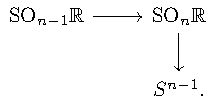
\includegraphics{fiber-bundle-so}
  \]
\item Consider the action of $\SU_n$ on the sphere
  $S^{2n-1}\subset\bbC^n$. Then it is a homogeneous space, so we have a
  fiber bundle
  \[
    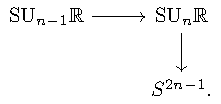
\includegraphics{fiber-bundle-su}
  \]
\end{enumerate}

In fact, action of $G$ can be used to define smooth structure on a
set. Indeed, if $M$ is a set (with no predetermined smooth structure) with
a transitive action of a Lie group $G$, then $M$ is in bijection with
$G/H$, $H\coloneq\Stab_G m$ and thus, by Theorem 2.11 $M$ has a canonical
structure of a manifold of dimension $\dim G-\dim H$.

\begin{example}
  Define a \emph{flag} in $\bbR^n$ to be a sequence of subspaces
  \[
    \{0\}\subset V_1\subset V_2\subset\dotsb\subset V_n=\bbR^n,\qquad \dim
    V_i=i.
  \]
  Let $\calF_n(\bbR)$ be the set of all flags in $\bbR^n$. It turns out
  that $\calF_n(\bbR)$ has a canonical structure of a smooth manifold which
  is called the \emph{flag manifold}. The easiest way to define it is to
  note that we have an obvious action of the group $\GL_n\bbR$ on
  $\calF_n(\bbR)$. This action is transitive: by a change of basis, any flag
  can be identified with the standard flag
  \[
    V^{\text{std}}\coloneq\left( \{0\}\subset\Span(\bfe_1
      )\subset\Span(\bfe_1,\bfe_2
      )\subset\cdots\subset\Span(\bfe_1,\dotsc,\bfe_n )=\bbR\right)
  \]
  where $\langle \bfe_1,\dots,\bfe_n \rangle$ is the standard basis for
  $\bbR^n$. Thus, $\calF_n(\bbR)$ can be identified with the coset space
  $\GL_n\bbR/B_n\bbR$ where $B_n\bbR\coloneq\Stab V^{\text{std}}$ is the
  group of all invertible upper-triangular matrices. Therefore, $\calF_n$
  is a manifold of  dimension $n^2-n(n+1)/2=n(n-1)/2$.
\end{example}

%%% Local Variables:
%%% mode: latex
%%% TeX-master: "../MA598-Lie-Groups"
%%% End:


%% Bibliography
\bibliographystyle{plain}
\bibliography{lie-bib}
% \printindex
\end{document}

%%% Local Variables:
%%% mode: latex
%%% TeX-master: t
%%% End:
